\chapter{The Design of {\opp}}
\label{cha:the-design-of-omnet}

\section{Structure of an {\opp} executable}

Consider the following diagram:

\begin{figure}[htbp]
  \begin{center}
    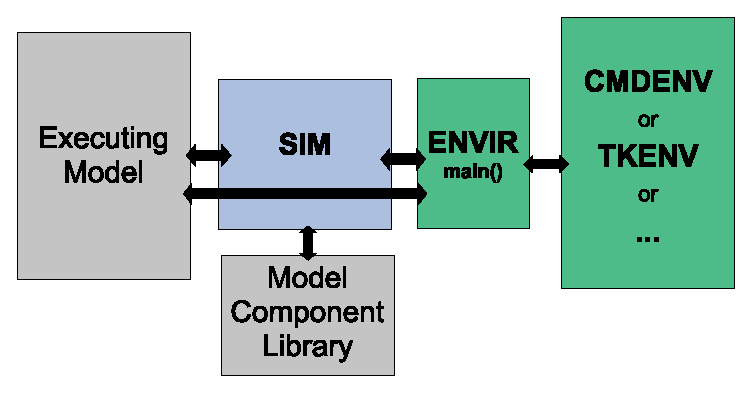
\includegraphics[width=4.757in, height=2.412in]{figures/usmanFig18}
    \caption{Architecture of {\opp} simulation programs}
  \end{center}
\end{figure}

A simulation program contains the simulated network (with its
simple\index{module!simple} and compound\index{module!compound}
modules etc.), SIM, ENVIR and exactly one of CMDENV and TKENV. SIM
contains the simulation class library\index{simulation!class library}
and the simulation kernel. The model only interacts with
SIM\footnote{the only exception is textual module output: it is sent
  directly to ENVIR: ev\texttt{<}\texttt{<}''hello''; ev.printf(''
  world'');}. ENVIR contains code that is common for all user
interfaces, and provides infrastructure like ini file handling for
them. \fname{main()} is also in ENVIR. Specific user interface code is
contained in CMDENV and TKENV. The above components are also
physically separated: they are in separate source directories and form
separate library files (\ttt{libsim\_std.a}, \ttt{libenvir.a} etc.)

The simulation program may contain several linked-in model
components\index{model!components}: networks,
simple\index{module!simple} module types,
compound module types, channel types etc. Any
network (but only one at a time) can be set up for simulation which
has all necessary components linked in.





\section{Embedding {\opp}}

Embedding is a special issue\index{simulation!embedding}. You probably
do not want to keep the appearance of the simulation program, so you
do not want Cmdenv and Tkenv. You may or may not want to keep ENVIR.

What you'll absolutely need for a simulation to run is the SIM
package. You can keep ENVIR if its philosophy and the infrastructure
it provides (\ttt{omnetpp.ini}, certain command-line options etc.)
fit into your design. Then the embedding program will take the
place of Cmdenv and Tkenv.

If ENVIR does not fit your needs (for example, you want the model
parameters to come from a database not from \ttt{omnetpp.ini}), then you
have to replace it. Your ENVIR replacement (the embedding program,
practically) must implement the \cclass{cEnvir} member functions from
\ttt{envir/cenvir.h}, but you have full control over the simulation.

Normally, code that sets up a network or builds the internals of a
compound module comes from compiled NED source.  You may not like the
restriction that your simulation program can only simulate networks
whose setup code is linked in. No problem; your program can contain
pieces of code like what is generated by nedc and then it can build
any network whose components (primarily the simple modules) are linked
in. Moreover, it is possible to write an integrated environment where
you can put together a network using a graphical editor and right
after that you can run it, without intervening NED compilation and
linkage.





\section{The simulation kernel}

The source code for the simulation kernel\index{simulation!kernel} of
{\opp} and the library classes reside in the sim directory.

Almost all objects are derived from \cclass{cObject} which
provides a common interface for them.





\subsection{The central object: cSimulation simulation}

The \cclass{cSimulation} class stores a network and manages simulation.
There is only one instance, a global object called \ttt{simulation}.
The object has two basic roles:
\begin{itemize}
  \item{as a vector of modules}
  \item{holds global variables (for example, the message queue).}
\end{itemize}





\subsection{Module classes}

Base class for module classes: \cclass{cModule}. Two derived classes:
\cclass{cCompoundModule}, \cclass{cSimpleModule}.  User simple
modules\index{module!simple} are derived from \cclass{cSimpleModule}.

A \cclass{cModule} has: array of parameters, array of gates + member
functions to set up and query parameters and gates.

\cclass{cSimpleModule} adds: put-aside queue, list of local objects + the
virtual function \fname{activity()} + member functions like
\fname{send()}, \fname{receive()} etc.

Gates are represented by the \cclass{cGate} objects.
Connections are not real objects: their attributes (delay, error,
datarate) are managed by the connection's source gate.





\subsection{Global registration lists}

There are global objects holding lists of components available
in an {\opp} executable. These lists are:


\begin{longtable}{|p{2cm}|p{4,3cm}|p{7.3cm}|}
\hline
%% ROW 1
\tabheadcol
\textbf{List object}
&
\textbf{\mbox{Macro that creates a}}\linebreak
\textbf{member.} \linebreak\linebreak
\textbf{Class of members}
&
\textbf{Function} \\\hline
%% ROW 2
\ttt{\cclass{cHead}}  \linebreak
\ttt{ networks;}
&
\ttt{\fmac{Define\_Network()}} \linebreak
\linebreak
\ttt{\cclass{cNetworkType}}
&
{\raggedright List of available networks\index{network!list of}.\\
A \cclass{cNetworkType} object holds a pointer to a function that can
build up the network.\\
\fmac{Define\_Network()} macros occur in the code generated by the NEDC
compiler.}\\\hline
% ROW 3
\ttt{\cclass{cHead}} \linebreak
\ttt{ modtypes;}
&
\ttt{\fmac{Define\_Module()},} \linebreak
\ttt{\fmac{Define\_Module\_Like()},}  \linebreak
\linebreak
\ttt{\cclass{cModuleType}}
&
{\raggedright List of available module types.\\
A \cclass{cModuleType} object knows how to create a module of a specific
type. If it is compound, it holds a pointer to a function that can
build up the inside.\\
Usually, \fmac{Define\_Module()} macros for compound modules occur in
the code generated by the NEDC compiler; for simple modules,
the \fmac{Define\_Module()} lines are added by the user.}\\\hline
%% ROW 4
\ttt{\cclass{cHead}} \linebreak
\ttt{ classes;}
&
\fmac{Register\_Class()} \linebreak
\linebreak
\ttt{ClassRegister}
&
{\raggedright List of available classes of which the user can create
  an instance.\\
A \cclass{cClassRegister} object knows how to create an (empty) object of a specific class.\\
The list is used by the \fname{createOne()} function that can create an
object of any (registered) type from a string containing the class
name. (E.g. \ttt{ptr = createOne( ``cArray'')} creates an empty
array.)\\
\fname{createOne()} is used by the PVM extension.\\
\fmac{Register\_Class()} macros are present in the simulation source
files for existing classes; has to be written by the user for new
classes.}\\\hline
%% ROW 5
\cclass{cHead} \linebreak
\ttt{ functions;}
&
\ttt{\fmac{Define\_Function()}} \linebreak
\linebreak
\ttt{\cclass{cFunctionType}}
&
{\raggedright List of mathematical functions.\\
A \cclass{cFunctionType} object holds a pointer to the function and knows
how many arguments it takes.}\\\hline
%% ROW 6
\cclass{cHead} \linebreak
\ttt{ linktypes;}
&
\fmac{Define\_Link()} \linebreak
\linebreak
\cclass{cLinkType}
&
{\raggedright List of link types.\\
A \cclass{cLinkType} object knows how to create \cclass{cPar} objects representing
the delay\index{channel!delay}, error\index{channel!error} and datarate\index{channel!datarate} attributes for a channel.\\
\fmac{Define\_Link()} macros occur in the code generated by the NEDC
compiler, one for each channel definition.} \\\hline
%% ROW 7
\ttt{\cclass{cHead}} \linebreak
\ttt{ locals;}
&
\ttt{-} \linebreak
\linebreak
\ttt{any object}
&
This is only `dummy' object, it stands for the current module's
local object list\\\hline
%% ROW 8
\ttt{\cclass{cHead}} \linebreak
\ttt{ superhead;}
&
\ttt{-} \linebreak
\linebreak
\ttt{\cclass{cHead}}
&
List of all other lists. \\\hline
\end{longtable}



\subsection{The coroutine package}

The coroutine package is in fact two coroutine
packages\index{coroutine}:

\begin{itemize}
  \item Portable coroutine package creates all coroutine stacks
     inside the main stack. It was taken from [KOF85]. It
     allocates stack by deep-deep recursions and then plays with
     \fname{setjmp()} and \fname{longjmp()} to switch from one another.

  \item On Windows, the Fiber functions (\fname{CreateFiber()},
     \fname{SwitchToFiber()}, etc) are used, which are part of
     the standard Win32 API.
\end{itemize}

The coroutines are represented by the \cclass{cCoroutine}
class. \cclass{cSimpleModule} has \cclass{cCoroutine} as one a
base class.





\subsection{Object ownership/contains relationships}

\textbf{Ownership:} Exclusive right and duty to delete the child
objects.  Ownership\index{ownership} works through \cclass{cObject}'s
ownerp/prevp/nextp and firstchildp/lastchildp pointers.


\textbf{'Contains' relationship:\index{contains relationship}} Only
for container classes, e. g.  \cclass{cArray} or \cclass{cQueue}.
Keeping track of contained objects works with another mechanism,
\textit{not} the previously mentioned ptrs. (E.g., \cclass{cArray}
uses a vector, \cclass{cQueue} uses a separate list).

The two mechanisms are \textit{independent}.

\textbf{What \cclass{cObject} does:}
\begin{itemize}
  \item{Owner of a new object can be explicitly given; if omitted,
    \fname{defaultOwner()} will be used.}
  \item{An object created through the copy
    constructor\index{ownership!copy constructor} will have the same
    owner as original and does not \fname{dup()} or take objects owned
    by the original.}
  \item{Destructor calls \fname{free()} for owned objects (see later)}
\end{itemize}


\textbf{Rules for derived classes:}
\begin{itemize}
  \item{Objects contained as data members: the enclosing object should
    own them.}
\end{itemize}

\textbf{Rules for container objects derived from cObject:}
\begin{itemize}
  \item{they use the functions: \fname[take()]{take(obj)},
    \fname[drop()]{drop(obj)}, \fname[free()]{free(obj)}}
  \item{when an object is inserted, if \fname{takeOwnership()} is
    true, should take ownership of object by calling
    \fname[take()]{take(obj)}. \fname{takeOwnership()} defaults to
    true!}
  \item{when an object is removed, they should call
    \fname[drop()]{drop(obj)} for it if they were the owner.}
  \item{copy constructor copies should \fname{dup()} and take
    ownership of objects that were owned by the original.}
  \item{destructor doesn't need not call \fname{free()} for objects:
    this will be done in \cclass{cObject}'s destructor.}
\end{itemize}

The class \cclass{cHead} is special case: it behaves as a container,
displaying objects it owns as contents.




\section{The user interface}

The source code for the user interface of {\opp} resides in the
\texttt{envir} directory (common part) and in the \texttt{cmdenv},
\texttt{tkenv} directories.

The classes in the user interface are \textit{not} derived from \cclass{cObject},
they are completely separated form the simulation kernel.





\subsection{The main() function}

The \fname{main()} function of {\opp} simply sets up the user
interface and runs it. Actual simulation is done in
\fname{cEnvir::run()} (see later).





\subsection{The cEnvir interface}

The \cclass{cEnvir} class has only one instance, a global object
called \fvar{ev}:

\begin{verbatim}
cEnvir ev;
\end{verbatim}

\cclass{cEnvir} basically is only an interface, its member functions
hardly contain any code. \cclass{cEnvir} maintains a pointer to a
dynamically allocated simulation application object (derived from
\cclass{TOmnetApp}, see later) which does all actual work.


\cclass{cEnvir} member functions deal with four basic tasks:
\begin{itemize}
  \item{I/O for module activities; actual implementation is different
    for each user interface (e.g. stdin/stdout for Cmdenv, windowing
    in Tkenv)}
  \item{setting up and running the simulation application}
  \item{provides functions called by simulation kernel objects to get
    information (for example, get module parameter settings from the
    configuration file)}
  \item{provides functions called by simulation kernel objects to
    notify the user interface of some events. This is especially
    important for windowing user interfaces (Tkenv), because the
    events are like this: an object was deleted so its inspector
    window should be closed; a message was sent so it can be
    displayed; a breakpoint was hit.}
\end{itemize}




\subsection{Implementation of the user interface: simulation applications}

The base class for simulation application is \cclass{TOmnetApp}.
Specific user interfaces such as \cclass{TCmdenv},
\cclass{TOmnetTkApp} are derived from \cclass{TOmnetApp}.

\cclass{TOmnetApp}'s member functions are almost all virtual.
\begin{itemize}
  \item{Some of them implement the \cclass{cEnvir} functions
    (described in the previous section)}
  \item{Others implement the common part of all user interfaces (for
    example: reading options from the configuration files; making the
    options effective within the simulation kernel)}
  \item{The \fname{run()} function is pure virtual (it is different
    for each user interface).}
\end{itemize}

\cclass{TOmnetApp}'s data members:
\begin{itemize}
  \item{a pointer to the object holding configuration file contents
    (type \cclass{cInifile});}
  \item{the options and switches that can be set from the
    configuration file (these members begin with \ttt{opt\_})}
\end{itemize}

Concrete simulation applications:
\begin{itemize}
  \item{add new configuration options}
  \item{provide a \fname{run()} function}
  \sloppy
  \item{implement functions left empty in \cclass{TOmnetApp} (like
    \fname{breakpointHit()}, \fname{objectDeleted()}).}
\end{itemize}


%
% section{Writing inspectors for TkEnv}
%
% TBD
%

%%% Local Variables:
%%% mode: latex
%%% TeX-master: "usman"
%%% End:
